\subsubsection{把消息画出来：先准备一组能对照的数据}
\label{sec:ros2-visualization}

前面我们已经在终端和 rqt 的消息监视器里看见了字段。不过，坐标在不在抖、图像有没有变色、检测框是不是跟着目标走，盯着一屏数字就有些费眼睛了。接下来我们把同一组数据放到曲线、图像和三维窗口里看。以后调程序时，你就可以把“好像不对”变成更具体的判断：哪一条曲线变了，哪一个坐标系反了，或者哪一帧的标注没有对上。

rqt 是一组可以拼在同一窗口里的 ROS 插件，适合快速发布、查字段、画曲线和看图像；RViz2 擅长把 ROS 的坐标系、位姿、轨迹和图形消息放进三维场景；Foxglove 则把这些观测放到一个布局里，还能通过桥接连接机器人、回放录制文件，并在曲线上做换算和测量。我们先把数据源准备好，再分别打开它们。

\begin{example}[一份数据源，三种观察方式]
本卷的 \path{examples/ros2/visualization-demo} 不需要相机，直接生成一块左右移动的绿色色块，以及绕圆运动的目标。它每 0.1 秒发布一次，话题与用途如下。
\begin{center}
\begin{tabular}{p{0.23\linewidth}p{0.38\linewidth}p{0.31\linewidth}}
\toprule
话题 & 消息类型 & 用来看什么\\
\midrule
\path{/viz/signal} & \path{std_msgs/msg/}\newline\path{Float64} & 正弦曲线\\
\path{/viz/pose} & \path{geometry_msgs/msg/}\newline\path{PoseStamped} & 位置与四元数朝向\\
\path{/viz/twist} & \path{geometry_msgs/msg/}\newline\path{TwistStamped} & 速度向量与角速度\\
\path{/viz/path} & \path{nav_msgs/msg/}\newline\path{Path} & 最近 120 个位置\\
\path{/viz/image} & \path{sensor_msgs/msg/}\newline\path{Image} & 640×360 的 rgb8 原图\\
\path{/viz/markers} & \path{visualization_msgs/msg/}\newline\path{MarkerArray} & 球、箭头、轨迹与文字\\
\path{/viz/annotations} & \path{foxglove_msgs/msg/}\newline\path{ImageAnnotations} & 二维框、中心点与标签\\
\path{/viz/scene} & \path{foxglove_msgs/msg/}\newline\path{SceneUpdate} & Foxglove 原生三维实体\\
\path{/tf} & \path{tf2_msgs/msg/}\newline\path{TFMessage} & map 到 target 的坐标变换\\
\bottomrule
\end{tabular}
\end{center}

先在 Ubuntu 22.04 / Humble 环境中安装本节用到的工具。之前装了 desktop 的话，RViz2 和部分 rqt 插件可能已经有了，再执行安装会由 apt 检查。
\par\medskip\noindent\begin{minipage}{\linewidth}
\begin{tbash}
source /opt/ros/humble/setup.bash
sudo apt update
sudo apt install ros-humble-rqt ros-humble-rqt-graph \
  ros-humble-rqt-publisher ros-humble-rqt-topic \
  ros-humble-rqt-plot ros-humble-rqt-image-view \
  ros-humble-rviz2 ros-humble-foxglove-msgs \
  ros-humble-tf2-ros python3-pyqtgraph
cd /你的教材目录/02-专项技术栈/examples/ros2/visualization-demo
python3 data_node.py
\end{tbash}
\end{minipage}\par\smallskip
把 cd 后的路径换成你的实际目录；几个 Python 文件放在同一目录，直接运行即可，不需要再创建功能包。后面开出的终端都加载同一套 Humble 环境，通信域与发现范围也保持一致。先让这个终端持续运行，在另一终端用 \texttt{ros2 topic list -t} 找到上表的话题，再用 \texttt{ros2 topic echo /viz/pose --once} 确认能收到消息。

项目文件很少，data\_node.py 负责定时发布，另外三个文件分别填写三维 Marker、图像标注和 Foxglove 场景；demo.rviz 保存本节的显示配置。下面先把数据源的完整代码放出来，三种图形消息的代码留到讲它们时再看。
\begin{lstlisting}[language={}]
visualization-demo/
  README.md
  data_node.py
  markers.py
  annotations.py
  scene.py
  demo.rviz
\end{lstlisting}
\lstinputlisting[language=Python,basicstyle=\ttfamily\fontsize{9.5}{11.5}\selectfont,caption={data\_node.py：统一生成位姿、曲线与图像}]{examples/ros2/visualization-demo/data_node.py}

构造函数保存发布者、TF 广播器和定时器，回调每次只取一次时间，供这组消息共用。位置沿着半径 1 m 的圆运动，线速度是位置对时间的导数；ROS使用四元数用来表示朝向，orientation.z 的含义不是 yaw。最近 120 个位姿组成 Path，\texttt{map -> target} 的 TF 则告诉查看器目标坐标系在哪里。

图像部分直接填入 RGB 字节：每个像素三个字节，所以 step 是 $640\times3$，data 的长度是 $360\times\text{step}$。绿色色块已经在原图里，检测框和文字由另一条标注话题提供。这样我们可以分别检查“图像到了没有”和“算法结果对上了没有”。这里只用合成色块演示接口，后面的 OpenCV 章节再把它换成实际图像处理。
\end{example}

\begin{exercise}\label{ex:v2-ros-viz-source}
启动数据源，记录 pose、image 和 annotations 的类型与一组时间戳。根据图像的 width、height、encoding、step 判断 data 应有多少字节；说明为什么标注需要沿用这帧图像的时间，而不是算法算完后的时间。
\end{exercise}

\subsubsection{rqt：连线、曲线与图像都看一遍}
\label{sec:ros2-rqt-views}

刚才的 Message Publisher 与 Message Monitor 解决了“发了什么、收到了什么”。现在再补上三个常用插件。你可以运行 \texttt{rqt}，从 Plugins 菜单依次加入 Introspection 下的 Node Graph、Visualization 下的 Plot 和 Image View；不同版本的菜单排法可能稍有变化，按插件名找即可。插件窗口可以拖动并停靠，常用布局通过 Perspectives 保存，下次打开再恢复。

\begin{example}[把位置变化与图像变化同时看见]
保持数据源运行，在加载环境的终端里按需打开下面的独立窗口，每条启动命令各占一个终端。通用写法是 \texttt{ros2 run <包名> <程序名> [插件参数]}，rqt\_plot 后面接要画的数值字段。
\par\medskip\noindent\begin{minipage}{\linewidth}
\begin{tbash}
ros2 run rqt_graph rqt_graph
ros2 run rqt_plot rqt_plot \
  /viz/signal/data /viz/pose/pose/position/x
ros2 run rqt_image_view rqt_image_view /viz/image
\end{tbash}
\end{minipage}\par\smallskip

在 Node Graph 里点击刷新，选择显示节点与话题的模式，找到 viz\_demo 到各话题的连线。查看器自己也是订阅者，会出现在图中；如果打开了隐藏叶子话题或调试节点的选项，一些线可能被过滤掉。它适合查“谁连接谁”，具体数据仍要到 Monitor、Plot 和 Image View 中看。

Plot 的输入框填 \path{/viz/signal/data}，点加号添加曲线；再填 \path{/viz/pose/pose/position/x} 添加第二条。这里用斜线走到消息内部的数值字段，不能只填整个 Pose。两条曲线分别是 $\sin t$ 与 $\cos t$，幅值约为 1，相差四分之一个周期。点击暂停可以冻结显示，移除曲线用减号或曲线菜单；缩放后用自动缩放或重置视图找回数据。不同绘图库的按钮位置会有差别，切换到 PyQtGraph 后再检查图例和坐标轴。

图\ref{fig:ros2-rqt-plot} 是这份数据在 Humble 的 rqt Plot 插件中实际画出的结果。蓝线看 signal.data，红线看 pose.position.x，先找幅值与相位关系，再回到数值字段核对。截图使用 PyQtGraph，并放大图例字号以便在书页里阅读。
\begin{figure}[htbp]
  \centering
  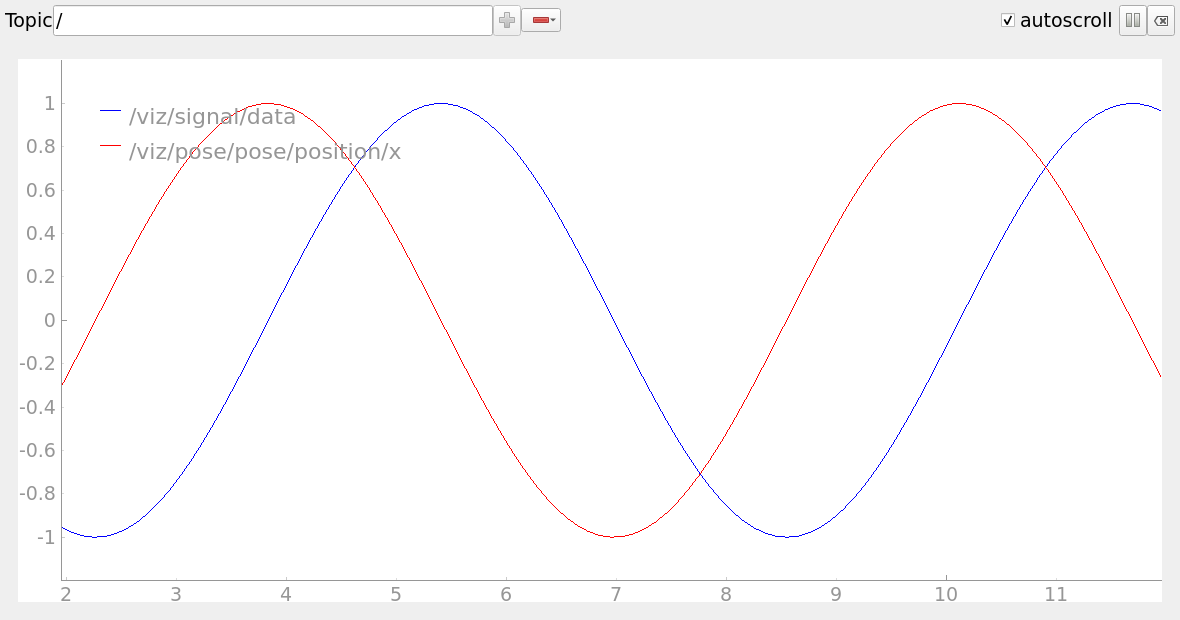
\includegraphics[width=\linewidth]{images/ros2_rqt_plot_revised.png}
  \caption{同一数据源的两条曲线：幅值约为 1，相差四分之一个周期}
  \label{fig:ros2-rqt-plot}
\end{figure}

Image View 的话题下拉框选择 \path{/viz/image}，传输方式使用 raw。你应看到深色背景上的绿色色块来回运动。调整窗口大小或缩放显示时注意保持纵横比，保存图像的按钮可以留下当前画面，后续对照算法结果会用得上。换到实际相机时，若驱动提供 compressed 传输，再选择对应方式；compressedDepth 用于深度图，不能当作普通彩色 JPEG 来选。

曲线空白时，先用 topic echo 确认字段有数据，再检查字段是不是数值、发布端是否仍在运行。图像空白时，检查话题类型和 QoS，并核对 encoding、step 与数据长度；红蓝颠倒往往是 RGB/BGR 顺序写错。rqt\_plot 使用自身的时间轴，不适合单凭两个窗口的横坐标判断传感器采集延迟。需要按消息时间对齐和测量时，我们下面用 Foxglove 再做一次。
\end{example}

\begin{exercise}\label{ex:v2-ros-rqt-views}
把 pose.position.y 加入曲线，与 x 对照，保存一张曲线和一帧原图。停止数据源，观察曲线与图像是否还保留最后结果，再重新启动。说明“窗口还有图”和“现在还在收到数据”有什么区别。
\end{exercise}

\subsubsection{RViz2：让坐标系、轨迹和图形各就各位}
\label{sec:ros2-rviz}

图像里的框只有像素位置，三维目标则还要说明相对于哪个坐标系。RViz2 的 Fixed Frame 是整个场景用来对齐数据的参考坐标系。比如消息写的是 camera，场景选的是 map，查看器就需要同一时刻从 camera 到 map 的 TF。本例的三维消息都写 map，并广播 map 到 target 的变换；图像的 camera\_optical 只用于二维原图显示，没有在这里假装完成相机外参标定。

\begin{example}[先手动加显示，再保存配置]
保持数据源运行，另开终端执行 \texttt{rviz2}。先在左侧 Global Options 中把 Fixed Frame 改成 \texttt{map}，再点 Add，按显示类型逐个添加：
\begin{center}
\begin{tabular}{p{0.20\linewidth}p{0.26\linewidth}p{0.46\linewidth}}
\toprule
显示类型 & 话题 & 观察结果\\
\midrule
Grid、TF & TF 订阅 /tf & 地面网格与 map、target 坐标轴\\
Pose & \path{/viz/pose} & 沿圆运动并转向的位姿箭头\\
Path & \path{/viz/path} & 最近 120 个位置连成的轨迹\\
MarkerArray & \path{/viz/markers} & 球、方向箭头、轨迹和文字\\
Image & \path{/viz/image} & 独立的二维原图窗口\\
\bottomrule
\end{tabular}
\end{center}
本例发布端使用 Reliable、Volatile、深度 10，先让各显示使用匹配的 QoS。接入常用的 Best Effort 相机或点云时，再在该显示的 Topic 属性中把 Reliability 调为 Best Effort。展开显示项的 Status 能看见错误原因；遇到 No transform 时先核对 frame\_id、时间戳和 TF 链，不要只把消息里的坐标系名字改成 map 来消掉提示。

视图选 Orbit，左键拖动旋转观察、滚轮拉近拉远；工具栏的 Move Camera 用于观察，Select 用于选中对象，Focus Camera 可以把视角移到目标附近。熟悉后通过 File / Save Config As 保存自己的 \texttt{.rviz} 文件。项目也提供了相同话题的配置，在项目目录中执行下面的命令即可恢复：
\par\medskip\noindent\begin{minipage}{\linewidth}
\begin{tbash}
rviz2 -d demo.rviz
ros2 run tf2_ros tf2_echo map target
\end{tbash}
\end{minipage}\par\smallskip
两个命令各占一个终端。前者打开显示，后者独立检查坐标变换；持续变化的平移和旋转应与场景中的 target 对应。Pose 是一份位置和朝向，Path 是一串带时间的位姿，TF 则连接坐标系，画面上看着相似的线和箭头，背后的消息各有用途。
图\ref{fig:ros2-rviz-views} 用提供的配置实际打开了这些显示。左上是原图，右边的蓝色球、切线方向箭头、黄色轨迹和 target 文字来自 MarkerArray；红色箭头来自 Pose，坐标轴来自 TF。
\begin{figure}[htbp]
  \centering
  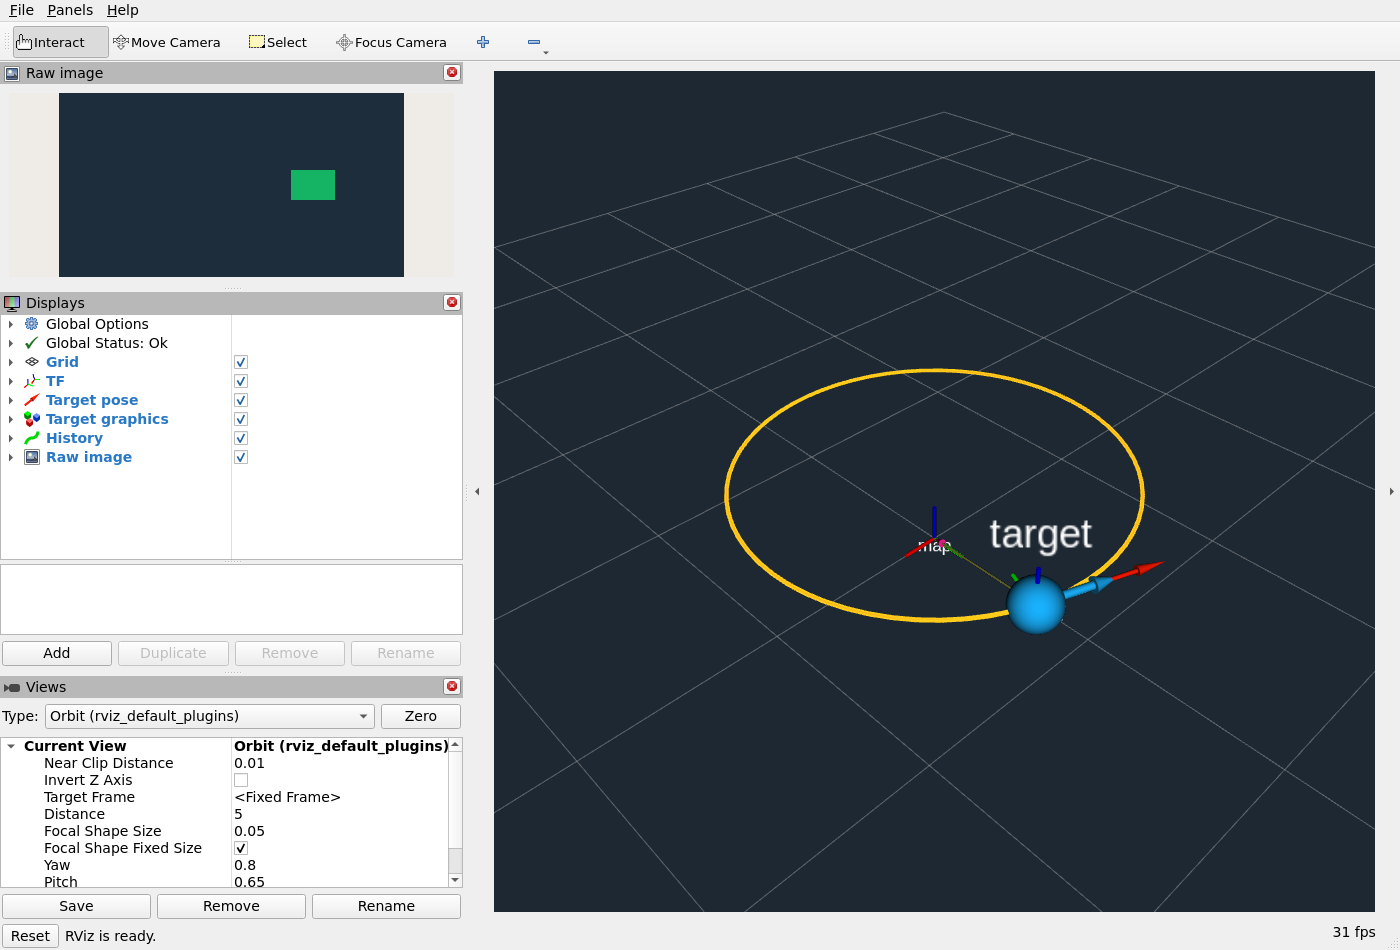
\includegraphics[width=\linewidth]{images/ros2_rviz_views_revised.png}
  \caption{Humble 中实际显示的原图、目标图形、位姿、轨迹与坐标轴}
  \label{fig:ros2-rviz-views}
\end{figure}
\end{example}

\subsubsection{Marker：绘制、更新与删除三维图形}
要给目标画一个球、给速度画一支箭头，或者在旁边放上编号，我们发布 \path{visualization_msgs/msg/Marker}。一次要更新多个图形时，把它们放进 MarkerArray.markers。RViz2 分别使用 Marker、MarkerArray 显示，Foxglove 的 3D 面板也能读取这两种 ROS 消息。

\begin{example}[球、箭头、轨迹和文字共用一份目标位置]
下面就是数据源调用的完整 markers.py。你可以对照每个图形的 type，再回到窗口找它。
\Needspace{8\baselineskip}
\lstinputlisting[language=Python,basicstyle=\ttfamily\fontsize{9.5}{11.5}\selectfont,caption={markers.py：填写并更新四种三维图形}]{examples/ros2/visualization-demo/markers.py}

\texttt{header.frame\_id} 决定坐标属于哪里，stamp 用来查相应时刻的 TF；pose 放图形的位置与朝向，单位四元数 \texttt{w=1} 表示不旋转。\texttt{ns} 和 id 一起标识图形，本例固定用 target 下的 0、1、2、3。下一次收到相同组合的 ADD，会更新已有图形，所以它能跟着目标移动；每帧都换一个新 id，则容易把过去的目标留满屏幕。

球的 scale 三个分量是三个方向的直径，CUBE 对应三个方向的边长；本例球的直径是 0.25 m。箭头可以用 pose 与长度表示，也可以像这里用 points 写出起点和终点；使用两点时，scale.x、y、z 分别控制箭杆直径、箭头直径和箭头长度。LINE\_STRIP 依次连接点，scale.x 是线宽；LINE\_LIST 每两个点画一段独立线，点数要成对。POINTS 用 scale.x、y 控制点的宽高，TEXT\_VIEW\_FACING 则用 scale.z 控制字高，内容填 text。

color 的 r、g、b、a 都在 0 到 1 之间，尤其别忘记 a：默认的 0 会让图形完全透明。给每个点设置 colors 时，数组长度要与 points 对应。需要网格模型还可以用 MESH\_RESOURCE 和 \texttt{package://包名/路径/model.dae} 等资源地址，先确认资源可被查看器读取，再考虑材质设置。更多图形类型可以查\href{https://github.com/ros2/ros2_documentation/blob/humble/source/Tutorials/Intermediate/RViz/Marker-Display-types/Marker-Display-types.rst}{Humble 的 Marker 类型说明}。

lifetime 设为 0 会一直保留，直到被更新或删除；本例设为 0.5 秒，每次更新重新计时，停止发布后就能看到图形消失。DELETE 删除同一个 ns/id，DELETEALL 清理该显示中的图形，通常不要在多人共用的话题上随手发送清空命令。\texttt{frame\_locked=true} 会让图形随着其 frame 的新 TF 移动；默认 false 按收到消息时的变换放置，是否持续跟随要按图形含义选择。

现在在另一终端切换本例的参数，先执行 false 并观察，再执行 true：
\par\medskip\noindent\begin{minipage}{\linewidth}
\begin{tbash}
ros2 param set /viz_demo show_target false
ros2 param set /viz_demo show_target true
\end{tbash}
\end{minipage}\par\smallskip
false 时 id 为 0 的球收到 DELETE，其他箭头、文字与轨迹继续显示；true 时再次 ADD 恢复球。这比只往消息数组里删掉球更明确：数组里没出现一个 id，并不表示查看器要删除它。
\end{example}

\begin{conclusion}
读三维画面时，我们要能回答三个问题：数据属于哪个坐标系，图形的尺寸和颜色有没有填对，同一个对象怎样更新和结束。TF 帮助对齐坐标，Marker 的 ns/id 帮助更新对象，lifetime 与删除动作帮助清理过期结果。它们都需要消息里的约定，查看器不会替我们猜。
\end{conclusion}

\begin{exercise}\label{ex:v2-ros-rviz-markers}
把球改成边长 0.25 m 的立方体，再改变颜色和寿命，记录结果。解释把 alpha 留成 0、每帧改 id、只从 MarkerArray 中移除一个元素各会发生什么；用 show\_target 演示明确删除与恢复。
\end{exercise}

\section{Foxglove：连接、观测与回放}
\subsubsection{Foxglove：安装、连接与保存自己的观察布局}
\label{sec:ros2-foxglove}

接下来我们把刚才分散的几个窗口放在一起。Foxglove 的桌面端与网页端使用相近的面板操作。桌面端安装在你用来观察数据的电脑，foxglove\_bridge 安装在运行 ROS 的环境里；通过桥接传过来的消息定义，如果是跨电脑，桌面端不必再装一整套相同的 ROS 工作空间。

\begin{example}[装好桌面端，再连接自己的数据源]
在 Ubuntu 22.04 中先用 \texttt{dpkg --print-architecture} 看架构，进入\href{https://foxglove.dev/download}{Foxglove 官方下载页}，选择 Linux 的 x64（amd64）或 arm64 包。把下载的 deb 放在 Downloads 中，用实际文件名安装：
\par\medskip\noindent\begin{minipage}{\linewidth}
\begin{tbash}
cd ~/Downloads
sudo apt install ./foxglove-studio-实际版本与架构.deb
\end{tbash}
\end{minipage}\par\smallskip
文件名可以用 Tab 补全，别把“实际版本与架构”原样输入。官方页面也给出 \texttt{sudo apt install ./foxglove-studio-*.deb} 的写法，使用通配符前先确认目录里只有本次要装的包。安装后从应用菜单打开 Foxglove；Windows/macOS 则在同页选对应安装包。桌面端后续更新按下载页的软件源说明执行。网页端可以直接打开 \url{https://app.foxglove.dev/}。

接着回到运行 Humble 的环境，保持数据源运行，在另一个终端安装并启动桥接：
\par\medskip\noindent\begin{minipage}{\linewidth}
\begin{tbash}
source /opt/ros/humble/setup.bash
sudo apt install ros-humble-foxglove-bridge
ros2 launch foxglove_bridge foxglove_bridge_launch.xml \
  address:=127.0.0.1 port:=8765
\end{tbash}
\end{minipage}\par\smallskip
本机练习把桥接监听在 127.0.0.1。Foxglove 中点 Open connection，选择 Foxglove WebSocket，地址填 \texttt{ws://localhost:8765}，再点 Open。连上后在 Topics 列表里找到 /viz 开头的话题，先加一个 Raw Messages 面板选择 /viz/pose，展开字段确认数据持续更新。

Foxglove 与 ROS 在不同电脑时，localhost 指的是查看器自己的电脑。这时把桥接的 address 参数设为 \texttt{0.0.0.0}。在可信实验网里，查看器填写机器人的实际 IP，例如 \nolinkurl{ws://192.168.1.20:8765}；这里的示例 IP 要换成你的地址，并核对端口与防火墙。这样实验服务会接受其他网卡上的连接，使用完按 Ctrl+C 关闭。

用 Add panel 添加 Raw Messages、Plot、Image 和 3D，可以拖动分隔线调整大小。把图像和三维场景放在一侧，曲线放在另一侧，就能边看目标边对照数值；各面板在左侧 Panel 设置中选择话题。调整好后打开 Layout 菜单，右键自己的布局，点 Save changes（保存更改），再用 Export（导出）留下 JSON 文件。队友导入后就能看到同样的面板和字段。自己的账号与版本决定布局存到个人还是团队，先确认保存位置。

本项目也附有 \texttt{foxglove-panels/} 中的面板配置。想先得到和示例一致的画面，可以在相应面板的设置页打开右上角菜单，选 Import/Export settings（导入/导出设置），粘贴该面板的 JSON 并应用；这一步只恢复选中的面板，最后仍要保存整个布局。下面我们逐个试清楚这些设置。
\end{example}

\subsubsection{Foxglove：给数字状态标注名称}
\begin{note}
“Annotate” 还有一种常见用法：给消息里的数字状态标上名字。比如 mode=1 到底表示待机还是跟踪？可以在自己的接口包（这里取名 viz\_interfaces）中写下面两份完整消息定义，再按前面自定义接口的步骤把它们加入 rosidl\_generate\_interfaces，重新构建并加载 install 环境。
\begin{lstlisting}[language={}]
# msg/Mode.msg
uint8 IDLE=0
uint8 TRACKING=1
uint8 LOST=2
\end{lstlisting}
\begin{lstlisting}[language={}]
# msg/TargetState.msg
viz_interfaces/Mode mode_foxglove_enum
uint8 mode
\end{lstlisting}
带 \texttt{\_foxglove\_enum} 后缀的字段紧挨在 mode 前面，给 Foxglove 提供常量定义；发布时仍给 mode 填 0、1、2。Raw Messages 与 State Transitions 可以同时展示数字和名字，曲线仍直接取 \texttt{.mode}。ROS2 中只有常量的 Mode 消息会带一个序列化填充字节，这不是只改注释就能完成的显示设置。另一种写法是在 Mode 中增加 \texttt{uint8 data}，外层使用 \texttt{viz\_interfaces/Mode mode}，此时数值路径变为 \texttt{.mode.data}。这里的状态名标注与后面画在图像上的 ImageAnnotations 各有用途，定义方式见\href{https://docs.foxglove.dev/docs/visualization/annotate-ros-enum-fields}{官方枚举标注说明}。

\begin{figure}[H]
  \centering
  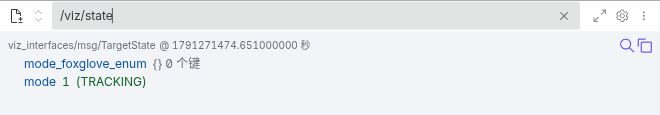
\includegraphics[width=0.9\linewidth]{images/ros2_foxglove_enum_revised.jpg}
  \caption{Humble 构建上述接口后发布 mode=1，Raw Messages 同时显示数字 1 与 TRACKING；常量定义字段本身仍是空对象。}
  \label{fig:ros2-foxglove-enum}
\end{figure}
\end{note}

\subsubsection{Foxglove Plot：字段路径与数值换算}
\label{sec:ros2-foxglove-plot}

先在 Plot 中把 X-axis value type 选为 Timestamp，添加两个 Series，Y-value 分别填 \path{/viz/signal.data} 和 \path{/viz/pose.pose.position.x}。Foxglove 用点号进入字段，与刚才 rqt\_plot 的斜线路径不同。输入路径时可以使用字段补全，也可以在 Raw Messages 中先确认字段层级，再复制相应路径。

\begin{example}[不用改发布程序，把四元数画成角度]
给 Plot 再加一条曲线，Y-value 填下面的完整路径。\texttt{.@rpy} 放在四元数对象后，转换结果还有 roll、pitch、yaw 三个字段，我们继续选 yaw，再把弧度换成角度。
\begin{lstlisting}[language={}]
/viz/pose.pose.orientation.@rpy.yaw.@degrees
\end{lstlisting}
这里只有 yaw 旋转，曲线会不断增长，到角度的表示边界后跳回另一端；这次跳变来自角度的周期表示，不表示目标突然转了整圈。真实三维姿态涉及旋转顺序，\texttt{.@rpy} 按 XYZ 内禀顺序转换，\texttt{.@ypr} 按 ZYX 顺序转换，先确认你要比较的角度定义。直接画 orientation.z 得到的只是四元数的一个分量。

这些后缀是 Foxglove 的字段路径函数（当前文档称 FoxQL），对查看器里的值做变换。常用写法整理如下，具体函数和版本差异可查\href{https://docs.foxglove.dev/docs/visualization/foxql}{官方函数说明}。
\begin{center}
\begin{tabular}{p{0.35\linewidth}p{0.57\linewidth}}
\toprule
字段后缀 & 用法与条件\\
\midrule
\nolinkurl{.@rpy.yaw}、\nolinkurl{.@rpy.roll} & 从 x/y/z/w 四元数中取欧拉角，结果是弧度；可继续选 pitch。\\
\nolinkurl{.@degrees}、\nolinkurl{.@radians} & 弧度转角度、角度转弧度，输入单位要先确认。\\
\nolinkurl{.@abs}、\nolinkurl{.@negative} & 取绝对值、改变符号，方便检查误差幅值或轴向。\\
\nolinkurl{.@mul(1000)}、\nolinkurl{.@div(1000)} & 乘除常数，例如米转毫米、毫秒转秒。\\
\nolinkurl{.@add(1)}、\nolinkurl{.@sub(1)} & 加减常数，用于比较带固定偏置的量。\\
\nolinkurl{.@norm} & 对 x/y/z 向量或数值数组取欧氏模长，例如速度大小。\\
\nolinkurl{.@length} & 取数组长度，例如 Path 中当前保存的位姿数。\\
\nolinkurl{.@sqrt}、\nolinkurl{.@log10} & 平方根、十进制对数，先检查输入取值范围。\\
\nolinkurl{.@sin}、\nolinkurl{.@cos} & 三角函数，输入使用弧度。\\
\nolinkurl{.@delta} & 相邻样本的值之差，结果单位与原值相同。\\
\nolinkurl{.@derivative} & 相邻样本的差除以时间差，单位变成原单位每秒。\\
\nolinkurl{.@timedelta} & 相邻样本之间的时间差，单位是秒。\\
\bottomrule
\end{tabular}
\end{center}

\Needspace{8\baselineskip}
在本例中可以直接试下面几条路径：
\begin{lstlisting}[language={}]
/viz/signal.data.@abs
/viz/pose.pose.position.x.@mul(1000)
/viz/twist.twist.linear.@norm
/viz/path.poses.@length
/viz/pose.pose.position.x.@derivative
/viz/pose.pose.position.x.@timedelta
\end{lstlisting}
第一条把正弦波的负半轴翻上来；第二条把米换成毫米；第三条的速度大小接近 1 m/s；第四条增加到 120 后保持不变。第五条可以与 \path{/viz/twist.twist.linear.x} 对照，差分会有离散采样误差；第六条约为 0.1 秒。函数可以顺序组合，例如先 \texttt{.@rpy.yaw} 再 \texttt{.@degrees}，每一步都接收上一步的结果。

取数组中的一项用 \texttt{[0]}，取全部用 \texttt{[:]}，例如 \path{/viz/markers.markers[0].pose.position.x}。把许多数组元素一起画进一条时间曲线，可能会在每个时刻连出一堆折线；想观察一个目标时，先选固定项或按 id 过滤。图形对象的数组顺序可能变化，工程里更可靠的路径是 \path|/viz/markers.markers[:]{id==0}.pose.position.x|，先在 Raw Messages 核对筛选结果，再加到曲线。

\begin{note}
\texttt{.@delta}、\texttt{.@derivative}、\texttt{.@timedelta} 需要 Timestamp 横轴，不能用在 XY 或 Array index 横轴上；一条函数链最多用一个这样的时间序列函数。函数缺失或路径报错时先检查客户端版本。用差分看角速度时，还要处理角度绕回和噪声，否则 $179^\circ$ 到 $-179^\circ$ 的表示变化会产生很大的假尖峰。
\end{note}

\end{example}

\subsubsection{Foxglove Plot：时间对齐与两点测量}
\begin{example}[按同一种时间来源比较曲线与轨迹]
消息里有正确填写的 \texttt{header.stamp} 时，我们\textbf{优先用它来画曲线}。在 Series 的 Timestamp 设置中选择 Header stamp（中文界面为“ROS 头时间戳”），这样比较的是数据采集或生成的时刻。传输和处理有延迟时，两条本来同时采集的数据也能按原来的时间对齐；\texttt{.@derivative} 和 \texttt{.@timedelta} 同样使用这里选定的时间来源。

本例的 pose、twist 和 path 都有 header，因此共同选 Header stamp；Float64 没有 header，signal 使用 Log time。这里先用它对照波形；真要精确比较 signal 与位姿的相位，就给自定义信号消息增加 Header，在同一次采样填入相同时间，再统一选 Header stamp。Log time 在实时连接中表示消息被接收的时刻，在录制文件中是原来的记录时刻，适合从接收侧观察消息间隔。先在 Raw Messages 确认 header.stamp 有效、持续更新，并核对比较对象使用同一种时钟；全为零或填错时，先修发布端。比较多条曲线时别混用采集时间与接收时间，采样频率不一样时也别把提示框中的最近一次值当成同一时刻的新样本。

现在点 Plot 工具栏中的 Inspection（两点检查）工具，依次选择两个曲线点。图例区域会显示两点的坐标以及沿各轴的差值：时间曲线的 $\Delta x$ 是时间间隔，$\Delta y$ 是数值变化。比如同一条正弦曲线的两个相邻峰值，间隔应该约为 $2\pi$ 秒。按 Esc 取消已选点，再按一次退出工具。

\begin{figure}[H]
  \centering
  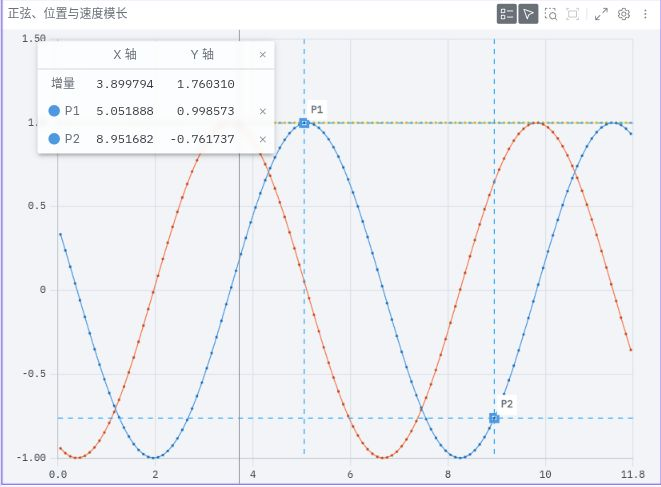
\includegraphics[width=0.96\linewidth]{images/ros2_foxglove_plot_measure_revised.jpg}
  \caption{打开点检查后选中 P1、P2；本次实测横轴差约 3.900 s，正弦值差约 1.760，两项单位分别读。}
  \label{fig:ros2-foxglove-plot-measure}
\end{figure}

还可以把 X-axis value type 改成 Expression，X-value 填 \path{/viz/pose.pose.position.x}，Y-value 填 \path{/viz/pose.pose.position.y}，Time range 选 All，Axis scales 选 1:1。这样会画出平面上的圆轨迹，两轴单位都是米，用两点检查还可以读到直线距离。时间曲线的横轴是秒、纵轴是米时，沿两轴的差值各有用途，把它们合成一个“距离”就没有物理意义了。

\begin{figure}[H]
  \centering
  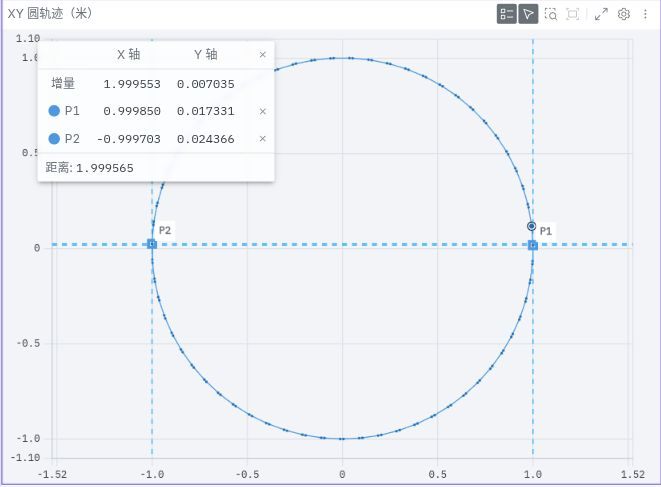
\includegraphics[width=0.96\linewidth]{images/ros2_foxglove_xy_measure_revised.jpg}
  \caption{XY 图的两轴都取位置，等比例显示圆轨迹；选取接近相对的两个采样点，实测距离为 1.999565 m。}
  \label{fig:ros2-foxglove-xy-measure}
\end{figure}

滚轮缩放、拖动平移，选中面板后按 r 或双击重置视图；按 z 进入框选缩放。按住 Alt 只缩放横轴，Shift 只缩放纵轴。曲线比较多时给 Series 改一个带单位的 Label，必要时分到不同面板或第二纵轴；右键图表导出 CSV，保留字段路径、时间来源和单位，后面复查才知道画的是什么。完整操作见\href{https://docs.foxglove.dev/docs/visualization/panels/plot}{官方 Plot 面板说明}。
\end{example}

\begin{exercise}\label{ex:v2-ros-foxglove-plot}
画出 yaw 的角度曲线、速度模长和相邻消息时间差。用 Inspection 测量正弦曲线两个相邻峰值的间隔，再用 XY 图测量圆上相对两点的距离。记录表达式、时间来源和单位，解释为什么时间曲线上的两轴差值不能直接合成空间距离。
\end{exercise}

\subsubsection{Foxglove 的 Image：把检测框与原图对上}
\label{sec:ros2-image-annotations}

先在 Image 面板选择 \path{/viz/image}。绿色色块应该和 rqt 中一样，但检测框不会因为你有一条“包含四个点的普通消息”就自动出现。Foxglove 识别的是明确的标注类型，这里使用 \path{foxglove_msgs/msg/ImageAnnotations}，里面按用途放 circles、points 和 texts。它们属于像素坐标，原点在图像左上角，x 向右、y 向下，和刚才以米为单位的三维 Marker 分开填写。

\begin{example}[原图不动，框、中心与标签单独发布]
下面是完整的 annotations.py。四个角点组成 LINE\_LOOP，查看器自动连接最后一点与第一点；圆和文字分别用自己的标注类型，颜色仍要填 alpha。
\Needspace{12\baselineskip}
\lstinputlisting[language=Python,basicstyle=\ttfamily\fontsize{9.5}{11.5}\selectfont,caption={annotations.py：二维框、中心和标签}]{examples/ros2/visualization-demo/annotations.py}

box 的 points 是像素位置，thickness 是像素线宽，fill\_color.a 默认 0，框内保持透明；CircleAnnotation 的 diameter 是直径。TextAnnotation 的 position 是文字区域的左下锚点，整个图像坐标仍以左上为原点，font\_size 用像素表示。这里的 confidence 是为展示准备的固定文本，示例没有执行目标识别。

回到 Image 的 Panel 设置，在可用标注话题中勾选 \path{/viz/annotations}，确认它显示为 ImageAnnotations，再打开 General 中的 Sync timestamps。你应看到黄色框包住绿色色块，红色小圆标出中心，文字在框上方；关闭标注话题时，原图仍保留色块。原图可以选择适合窗口、1:1 像素等缩放方式，查看像素值时把显示缩放与原图坐标分清。

\begin{figure}[H]
  \centering
  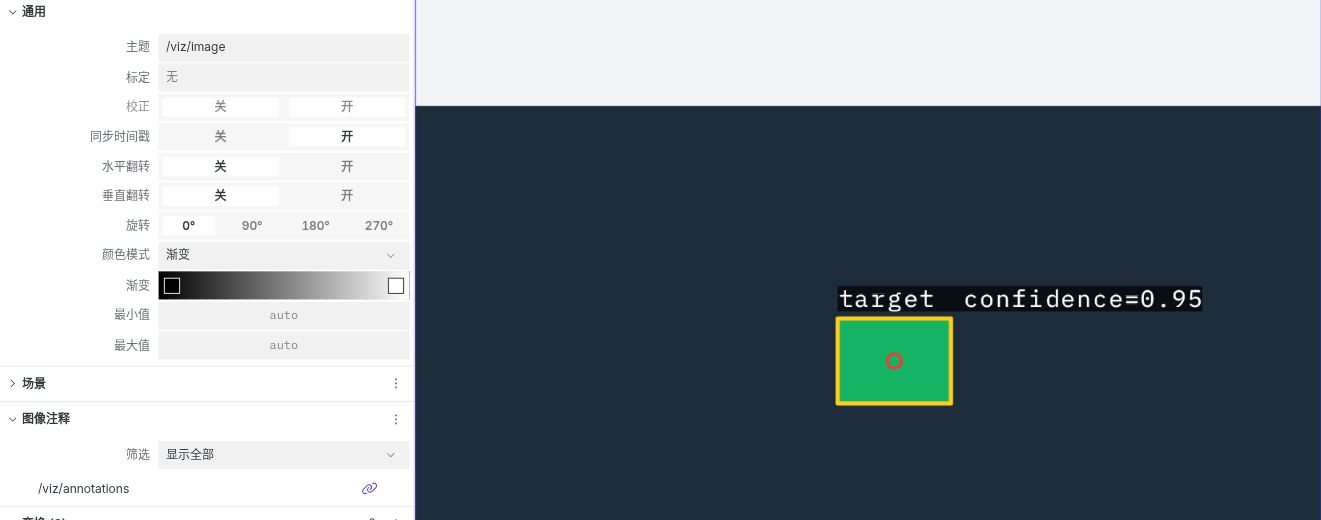
\includegraphics[width=0.96\linewidth]{images/ros2_foxglove_image_sync_revised.jpg}
  \caption{Image 面板打开时间戳同步，并启用 /viz/annotations；黄色框、红色中心与文字和原图一起显示。}
  \label{fig:ros2-foxglove-image-sync}
\end{figure}

同步匹配的是消息时间戳，不是“同样每秒发十次”。本例在同一次回调中把 image.header.stamp 传给每一个标注，新版 ImageAnnotations 的顶层 timestamp 也使用同一个值。算法稍晚算完时，仍把结果关联到输入图像的 header.stamp，别换成处理完成时的当前时间。旧版消息没有顶层 timestamp 时，客户端会使用标注元素的 timestamp，因此代码也给每一项填入同一时间。

打开同步后画面不更新，先检查是否只有框没有图、某个已勾选的标注话题停发，或两边时间差了一点；这里要求时间戳完全一致。本例把标注统一晚填 50 ms 后，客户端显示“等待同步消息”，恢复原图时间后又能正常更新。把检测框坐标按另一种图像尺寸计算，或者把归一化的 0 到 1 坐标直接填成像素，也会让框挤到角落里。前面合成图像的位移有意与圆运动分别定义，这些二维框用于演示像素标注，没有用相机模型把三维位置投影进图像。

真实相机的 CompressedImage 也可以在 Image 面板显示；需要叠加三维物体投影时，还要提供 CameraInfo 中的内参与坐标变换。单纯显示二维框不要求 CameraInfo；投影与畸变处理留到相机标定章节，别为了能看到框就随便填一份内参。像素标注、同步和投影的设置见\href{https://docs.foxglove.dev/docs/visualization/panels/image}{Image 面板说明}，字段类型见\href{https://docs.foxglove.dev/docs/sdk/schemas/image-annotations}{ImageAnnotations 定义}。
\end{example}

\begin{exercise}\label{ex:v2-ros-image-annotations}
把框的线宽改成 5 像素、中心圆直径改成 20 像素，保存一帧带标注的画面。再临时把所有标注时间戳加 50 ms，观察开启同步后的现象，恢复代码后重启。说明显示错误来自坐标、时间还是图像编码，并给出核对办法。
\end{exercise}

\subsubsection{Foxglove 3D：场景实体与空间测量}
\label{sec:ros2-foxglove-3d}

在 3D 的 Panel 设置里把 Display frame 选为 map，打开 TF、/viz/pose、/viz/path 与 /viz/markers，你应看到和 RViz2 对应的目标及轨迹。点一个对象可以查看其话题、编号与字段，再打开 Raw Messages 查同一对象。想跟着目标观察时可以选择 target 为跟随的坐标系；先用 map 看清整个运动，再切换视角，避免把相机视角的变化误认成目标运动。

\begin{example}[一个 SceneEntity 组合多个三维图形]
ROS Marker 可以直接共用，Foxglove 也提供原生的 \path{foxglove_msgs/msg/SceneUpdate}。它的 entities 中每个 SceneEntity 都有 frame\_id、timestamp、字符串 id、lifetime 和 frame\_locked，再把方块、箭头、线、文字等放到 cubes、arrows、lines、texts 数组中。下面的 scene.py 在同一个实体里组合一个方块和一段文字。
\lstinputlisting[language=Python,basicstyle=\ttfamily\fontsize{9.5}{11.5}\selectfont,caption={scene.py：把多个图元组合成一个三维实体}]{examples/ros2/visualization-demo/scene.py}

在 3D 中关闭 /viz/markers，打开 /viz/scene，绿色方块与文字就来自这份消息。cube 的 pose 给位置与朝向，size 给三轴尺寸；text.billboard 让文字朝向查看相机，scale\_invariant 让 font\_size 按屏幕像素表示，否则字高按世界坐标中的尺寸解释。本例每次沿用 target 这个 id，在同一话题中替换已有实体，lifetime 为 0.5 秒，停止更新后会过期。

SceneUpdate.deletions 可以放 SceneEntityDeletion，填写新时间、type 为 MATCHING\_ID、id 为 target，删除同话题中的旧实体；ALL 清理该话题已有实体。需要持续删除时先停止该实体的发布，否则下一条 entities 更新又会加回来。Marker 使用 ns/id 与 action，SceneUpdate 使用实体 id 和独立的 deletions 数组，各按自己的消息定义填写。RViz2 的默认显示不直接识别 SceneUpdate，使用哪种接口也要考虑队友的查看工具。

再点 3D 右侧的 Measure 工具，选择两个点读距离。默认点击落在地面平面上，测量实体表面或点云点时按住 Alt 启用吸附（macOS 用 Option），确认端点确实贴在对象上。世界坐标单位为米，量一个已知 0.25 m 的方块可以帮助检查尺度。测到的只是当前展示的几何结果；坐标变换或尺寸填错时，尺子也会跟着量错。图形接口与测量控制分别见\href{https://docs.foxglove.dev/docs/sdk/schemas/scene-update}{SceneUpdate 定义}和\href{https://docs.foxglove.dev/docs/visualization/panels/3d}{3D 面板说明}。
\end{example}

\subsubsection{MCAP 录制与回放：把一次观察留下来}
\begin{example}[录一段，再慢慢找不对劲的时刻]
实时数据太快时，我们先把它留下。Humble 默认常用的 db3 不保存全部自定义消息定义，这里安装 MCAP 存储插件，并明确使用 \texttt{-s mcap}。保持数据源运行，在新的工作目录中录制本例的话题：
\par\medskip\noindent\begin{minipage}{\linewidth}
\begin{tbash}
sudo apt install ros-humble-rosbag2-storage-mcap
mkdir -p ~/ros_viz_recordings
cd ~/ros_viz_recordings
ros2 bag record -s mcap -o viz_demo_01 \
  /viz/signal /viz/pose /viz/twist /viz/path /viz/image \
  /viz/markers /viz/annotations /viz/scene /tf
\end{tbash}
\end{minipage}\par\smallskip
录十几秒后按 Ctrl+C，让录制器正常收尾；输出目录要用尚不存在的名字，第二次可以改成 viz\_demo\_02。先用 \texttt{ros2 bag info viz\_demo\_01} 核对话题和消息数量，再关闭实时连接，在 Foxglove 用 Open local file(s) 打开目录里的 \texttt{.mcap} 文件，并恢复自己的布局。文件从容器产生时，先找到宿主能访问的实际路径。

回放可以暂停、拖动时间线、降低播放速度。点 Plot 上的一个时间点，回放位置会跳到那里，Image 和 3D 也跟着显示该时刻附近的数据。再用两点检查量周期、位置变化或处理异常持续多久；图像与标注开启同步时，查看同一帧的对应关系。实时模式没有“跳到刚才那一刻”的录制时间线，这也是我们要留下文件的原因。

\begin{figure}[H]
  \centering
  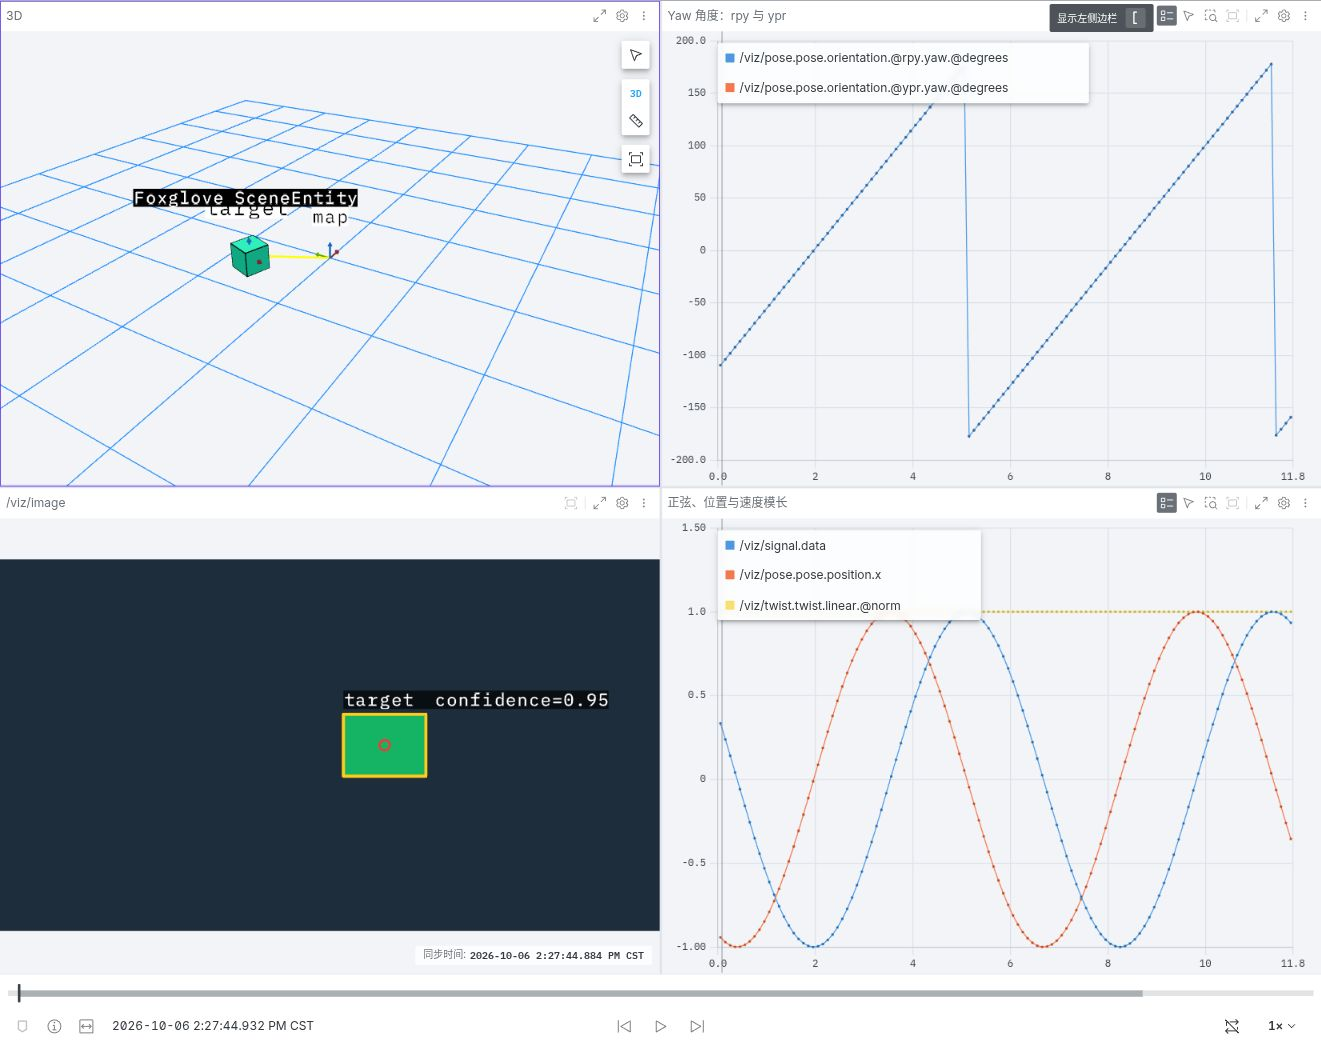
\includegraphics[width=0.98\linewidth]{images/ros2_foxglove_replay_revised.jpg}
  \caption{同一份 MCAP 的暂停画面：左侧对照 SceneEntity 和原图标注，右侧查看 yaw、位置与速度模长；下方时间线选择要复查的时刻。}
  \label{fig:ros2-foxglove-replay}
\end{figure}

录制与显示支路也会消费带宽、CPU 和存储。本节 640×360、10 Hz 的数据用来练工具；接上高帧率相机时，按后面的大图像链路章节安排降频观测支路，再检查显示或录制是否影响主链路。
\end{example}

\begin{conclusion}
现在我们有了几种互相补充的观察方式：先用消息字段确认输入，再用曲线看变化，用图像核对像素与标注，用三维场景核对坐标与尺寸，最后把有问题的过程录下来回放。保存画面时，也把话题、字段路径、时间来源、单位与显示配置留下来，队友才能复查你看到的现象。
\end{conclusion}

\begin{exercise}\label{ex:v2-ros-viz-replay}
保存一份包含 Plot、Image 和 3D 的布局，录制至少 10 秒 MCAP，重新打开文件。用同一时间点对照位姿曲线、目标图形和原图标注；提交布局、录制文件与一项测量结果，并说明这里哪些数据是合成的、哪些功能仍需接入实际相机后验证。
\end{exercise}
